\chapter{Testing and Results} \label{chap:testing_and_results}

\color{red} TODO: Write a nice intro to the chapter \color{black}

It was interesting to note the performance differences between the previous networks and the described two-phase network.

\section{Intensity Reconstruction}

\begin{figure}[htb]%
    \centering
    \subfloat[\centering]{{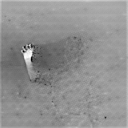
\includegraphics[width=0.18\textwidth]{implementation/images/dvs_wave_fluorescent_led.png}}}%
    \qquad
    \subfloat[\centering]{{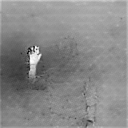
\includegraphics[width=0.18\textwidth]{implementation/images/dvs_wave_fluorescent.png}}}%
    \qquad
    \subfloat[\centering]{{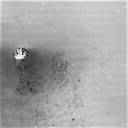
\includegraphics[width=0.18\textwidth]{implementation/images/dvs_wave_lab.png}}}%
    \qquad
    \subfloat[\centering]{{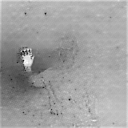
\includegraphics[width=0.18\textwidth]{implementation/images/dvs_wave_led.png}}}%
    \qquad
    \subfloat[\centering]{{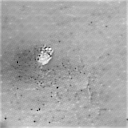
\includegraphics[width=0.18\textwidth]{implementation/images/dvs_wave_natural.png}}}%
    \caption{A waving motion being reconstructed from events captures by DVS128 event camera under different lighting conditions.The lighting conditions are as follows; \textbf{(a)} fluorescent led, \textbf{(b)} fluorescent, \textbf{(c)} lab lighting, \textbf{(d)} led lighting and \textbf{(e)} natural lighting.}%
    \label{fig:wave_in_lightings_reconstructions}%
\end{figure}

\color{red} TODO: Include image and explanations of reconstructions \color{black}

\subsection{NMNIST Dataset}

\subsection{DVS128 Gesture Dataset}

\section{Classification Results}

\begin{table}[htb]
    \centering
    \begin{tabular}{|| c | c | c ||}
        \hline
        Network     & NMNIST & DVS128 Gesture \\
        \hline \hline
        Conv3D Event Classifier          & 81.43\%   &   \color{red} 47.22\% \color{black}    \\
        \hline
        Conv2D LTSM Event Classifier         & 95.80\%   &        \\
        \hline
        Custom LTSM Event Classifier         & \color{red} 48.10\% \color{black}   &        \\
        \hline
        Conv2D LTSM Reconstruction Classifier           & \color{red} 83.13\% \color{black}    &    \color{red} 19.26\% \color{black}   \\
        \hline
    \end{tabular}
    \caption{A table showing classification accuracies of various models.}
    \label{tab:network_performances}
\end{table}